\documentclass[a4paper, 12pt]{article}
\usepackage{geometry}
\usepackage{float}
\usepackage{xcolor}
\geometry{margin=2cm}
\usepackage[indonesian]{babel}
\usepackage{setspace}
\onehalfspacing{}
\usepackage{hyperref}
\hypersetup{
    colorlinks,
    citecolor=black,
    filecolor=black,
    linkcolor=blue,
    urlcolor=blue
}

\definecolor {biru}{HTML}{1E66F5}
\definecolor {kuning}{HTML}{F6BF00}
\definecolor {abu}{HTML}{4C4F69}

\usepackage{graphicx}
\graphicspath{./images/}
\title{\textbf{Tugas Perorangan}\linebreak
\textbf{Tugas 5 Pembuatan Homepage STMIK Bandung}\linebreak}
\date{}

\usepackage{subfiles}
% \usepackage{indentfirst}
\setlength{\parindent}{20pt}
\begin{document}
\subfile{./subfiles/cover.tex}

% \tableofcontents
% \thispagestyle{empty}
% \pagebreak
% \clearpage
\setcounter{page}{1}
\section{Pendahuluan}
\href{https://www.figma.com/design/BTp5GY5lXf63dsjMJ1upku/Homepage?node-id=0-1&t=ly0hrx6yfXIWkYsS-1}{Link Homepage di Figma}\newline
\begin{figure}[h]
  \begin{center}
    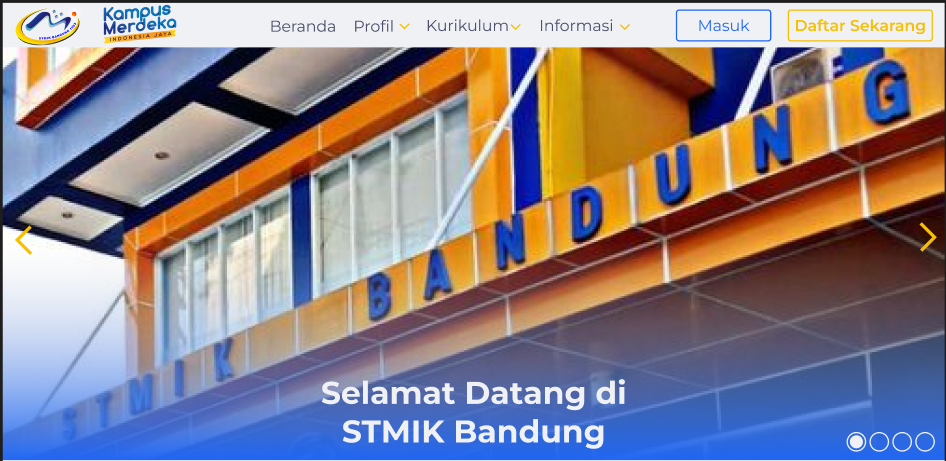
\includegraphics[width=0.95\textwidth]{images/gambar1.png}
  \end{center}
  \caption{tampilan utama dari Homepage STMIK Bandung}\label{fig:stmik}
\end{figure}
Berikut ini adalah penjelasannya:
\subsection{Penggunaan Warna}
untuk penggunaan warna yang diambil adalah warna biru sebagai warna utama dikarenakan warna biru adalah warna utama dari STMIK Bandung dan warna oranye sebagai warna pendukungnnya, dengan pallette warna seperti berikut:
\begin{itemize}
  \item \textcolor{biru}{1E66F5 :biru} Sebagai Warna utama
  \item \textcolor{kuning}{F6BF00 :Kuning} Sebagai Warna Pendukung
  \item \textcolor{abu}{4C4F69 :Abu-Abu} Sebagai Warna Text
  \item EFF1F5 :Putih Sebagai Warna Background
  \item FFFFFF :Putih Sebagai Warna overlay
\end{itemize}
\subsection{Bagian Navigasi}
Untuk bagian navigasi tersendiri dibagi menjadi 3 bagian berdasarkan posisi dari kiri ke kanan yaitu:
\begin{itemize}
  \item Logo STMIK Bandung untuk menjabarkan bahwa berada di website STMIK Bandung dan dapat kembali ke halaman utama jika ditekan
  \item Area navigasi halaman yang berada di tengah halaman yang berfungsi sebbagai navigasi cepat untuk pengguna untuk mengakses halaman lainnya 
  \item Area Pendaftaran dan login yang berfungsi untuk penginputan / masuk mahasiswa
\end{itemize}
\begin{figure}[H]
  \begin{center}
    
\includegraphics[width=0.95\textwidth]{images/gambar2.png}
  \end{center}
  \caption{Area Navigasi}\label{fig:navi}
\end{figure}

\subsection{Bagian halaman utama}
kemudian pada halaman utama menampilkan foto-foto STMIK Bandung untuk memberikan gambaran secara singkat bagaimana STMIK Bandung itu dengan cepat dan memiliki tombol navigasi untuk mengganti gambarnya dan bisa juga berganti dengan selang waktu yang di tentukan
\begin{figure}[H]
  \begin{center}
    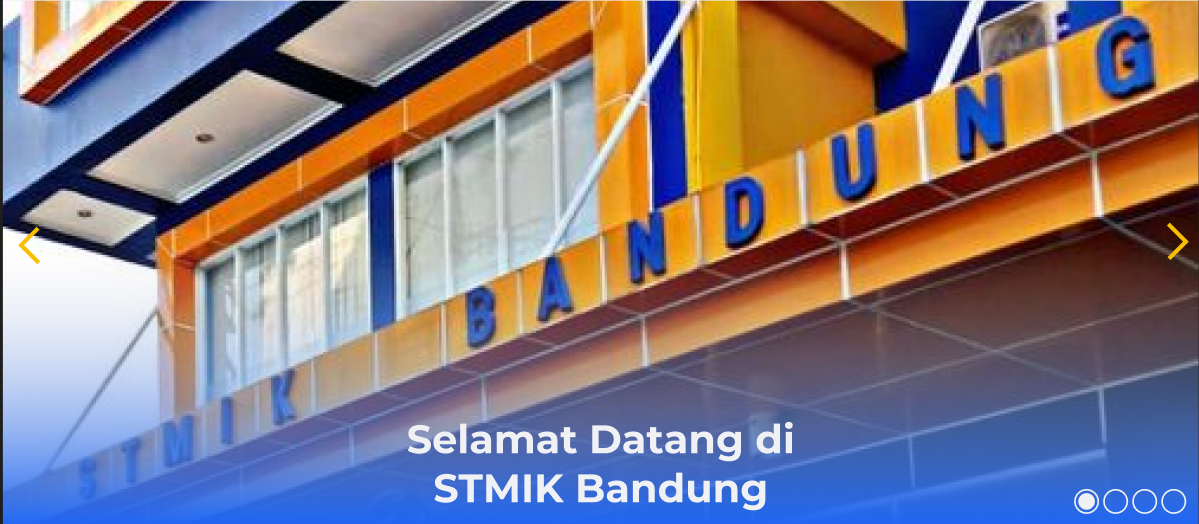
\includegraphics[width=0.95\textwidth]{images/gambar3.png}
  \end{center}
  \caption{Area halaman utama}\label{fig:}
\end{figure}

\subsection{Bagian Informasi Singkat}
dibawahnya ada section yang menampilkan informasi singkat mengenai kenapa kuliah di STMIK Bandung yang dapat membantu memperjelas lagi bagi pengunjung. 
\begin{figure}[H]
  \begin{center}
    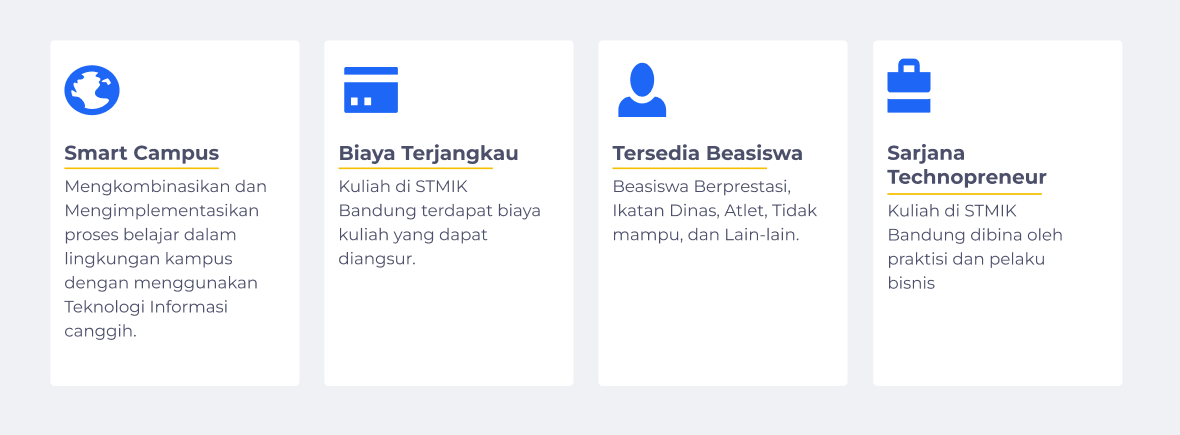
\includegraphics[width=0.95\textwidth]{images/gambar4.png}
  \end{center}
  \caption{Area Informasi Singkat}\label{fig:informasi}
\end{figure}

\subsection{Bagian Berita}
bagian ini menampilkan berita yang terjadi di kampus STMIK Bandung maupun informasi penting lainnya bagi mahasiswa / peserta didik baru. 
\begin{figure}[H]
  \begin{center}
    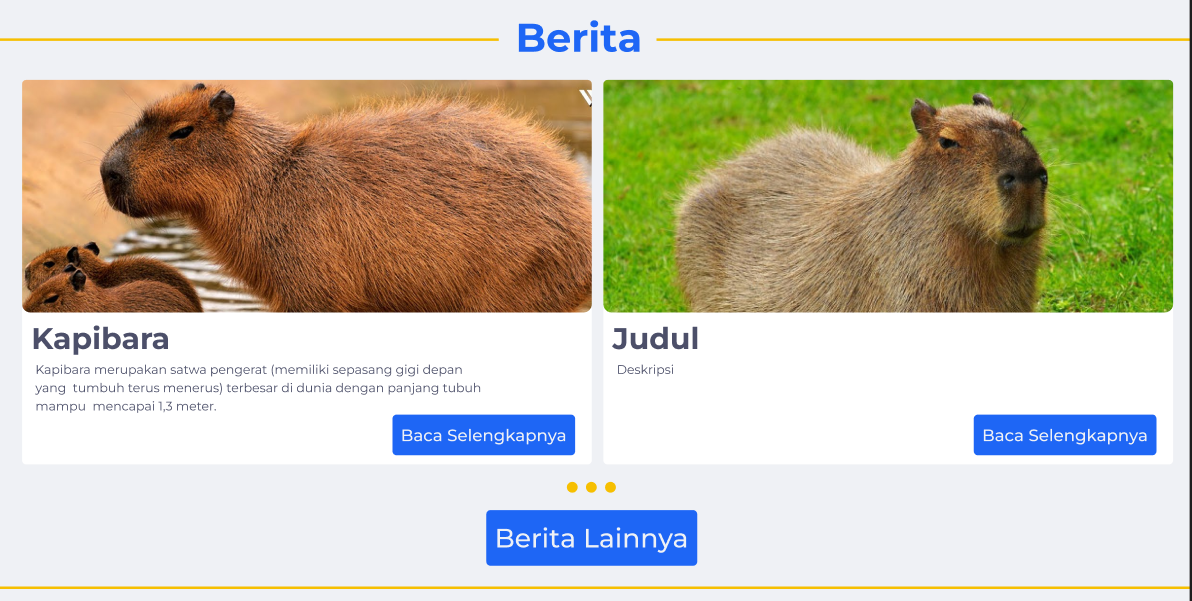
\includegraphics[width=0.95\textwidth]{images/gambar5.png}
  \end{center}
  \caption{Area Berita}\label{fig:berita}
\end{figure}

\subsection{Bagian Footer}
setelah itu pada bagian dibawah menampilkan informasi mengenai kontak info jika pengunjung memiliki pertanyaan lebih lanjut mengenai STMIK Bandung atau ingin mendaftar ke STMIK Bandung maka dapat dipandu oleh yang berwenang serta menampilkan tautan penting lainnya yang dapat membantu pengunjung mendapatkan informasi tambahan.
\begin{figure}[H]
  \begin{center}
    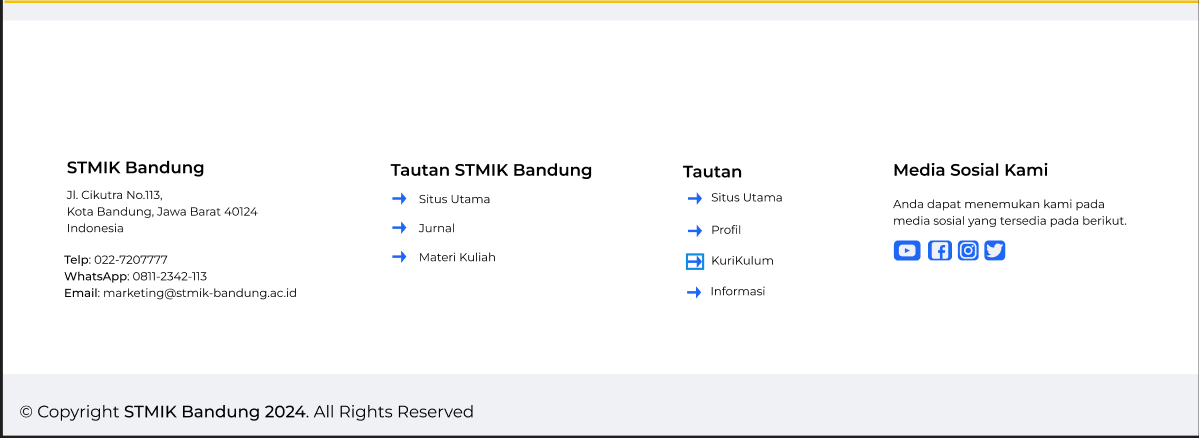
\includegraphics[width=0.95\textwidth]{images/gambar6.png}
  \end{center}
  \caption{Area Footer}\label{fig:footer}
\end{figure}

\end{document}
